\documentclass[12pt,a4paper]{report}
\usepackage{graphicx}
\usepackage{amsmath}
\usepackage{fancyhdr}
\usepackage{cite}
\usepackage{framed}
\usepackage{a4wide}
\usepackage{float}
\usepackage{epsfig}
\usepackage{longtable}
\usepackage{enumerate}
\usepackage{afterpage}
\usepackage{multirow}
\usepackage{ragged2e}
\usepackage{gensymb}
\usepackage{amsfonts} 
\usepackage[left=3.5cm,top=1.5cm,right=3cm,bottom=4cm]{geometry}
\usepackage{setspace}           
\usepackage{float}
\usepackage{txfonts}
\usepackage{lipsum}

\newcommand{\Usefont}[1]{\fontfamily{#1}\selectfont}

\usepackage{lscape} % for landscape tables
\renewcommand{\baselinestretch}{1.7} 

\usepackage{blindtext}
\usepackage{xpatch}
\usepackage{url}
\usepackage{leqno}
\usepackage{subcaption}

\linespread{1.5}
\usepackage[intoc, english]{nomencl}
\hyphenpenalty=5000
\tolerance=1000

\bibliographystyle{IEEEtran}
\renewcommand{\bibname}{References}
\nolistoftables
%*******************************************************************
%                        Header and Footer   
% This is not required in Technical reports submitted to CET ECE department.
% Please leave it commented                       
%*******************************************************************
%\pagestyle{fancy}
%\fancyhead{}
%\header and footer section
%\renewcommand\headrulewidth{0.1pt}
%\fancyhead[L]{\footnotesize \leftmark}
%\fancyhead[R]{\footnotesize \thepage}
%\renewcommand\headrulewidth{0pt}
%\fancyfoot[R]{\small College of Engineering Trivandrum}
%\renewcommand\footrulewidth{0.1pt}
%\fancyfoot[C]{2020 - 2021}
%\fancyfoot[L]{\small Title of the Seminar/Project}
%*******************************************************************


%*********************Figures*****************************
% Save all figures in the folder figures and include them in your 
% report using the command \includegraphics{figure-name}

\graphicspath{{figures/}}

% figure files can be in jpeg,jpg, png or pdf formats
%*******************************************************************


\begin{document}
	
	
%****The entries in this section are to be filled in by the student with appropriate values *************

% These values are used thoroughout the report 
% please fill in the appropriate values in the brackets {}

\gdef \title{SENSEAI } % Project title
%\gdef \author{Student Name}	 %student name

\gdef \degree{Software Requirement Specification} %degree
\gdef \branch{} %branch
\gdef \college{College of Engineering Karunagappally} % Name of the College
\gdef \collegeplace{Trivandrum} % Location of the College
\gdef \studentA{Abhijith H} %Project batch member 1
\gdef \studentAroll{KNP20CS002} % Project batch member 1 ktu id

\gdef \studentB{Anagha N } %Project batch member 2
\gdef \studentBroll{KNP20CS015} % Project batch member 2 ktu id

\gdef \studentC{Mishal K Nazeem} %Project batch member 3

\gdef \studentCroll{KNP20CS036} % Project batch member 3 ktu id

\gdef \studentD{Yethu Krishnan} %Project batch member 4
\gdef \studentDroll{KNP20CS052} % Project batch member 4 ktu id

\gdef \guide{Prof. Project guide} %Project guide
\gdef \guidedes{Assistant Professor}%project guide designation

\gdef \guideco{Prof. Project coguide} %Project coguide
\gdef \guidecodes{Assistant Professor}%project coguide designation

\gdef \guideext{Prof. Project ext guide} %Project external organisation guide
\gdef \guideextdes{Engineer/Scientist}%project external guide designation
\gdef \guideextorg{External guide organization} % Project external guide organization

\gdef \projcordinatorA{Prof. Project coordinator}% Project coordinator 1 
\gdef \projcordinatorAdes{Assistant Professor}% Project coordinator 1 designation

\gdef \projcordinatorB{Prof. Project coordinator 2} % Project coordinator 2 
\gdef \projcordinatorBdes{Assistant Professor}% Seminar coordinator 2 designation

\gdef \hod{Dr. Head of Dept} %Head of Department
\gdef \hoddes{Professor and Head} %HOD designation

\gdef \acadyear{2020 - 24} % Academic year
\gdef \month{April 2023} %Month of Report submission
\gdef \date{15-04-2023} %Date of signing the declaration

%*******************************************************************
% The font pages. The source tex files are there in the folder
%==================================coverpage.tex================================


\newenvironment{coverpage}
\thispagestyle{empty}
\begin{titlepage}
	\begin{center}
		{\Usefont{phv} \Large \bf \title \par}
		\vspace*{40pt}
		\large \em \Usefont{pzc}{ 
			 \par
			\\
			}\\ [.15\baselineskip] \par
		\Usefont{ppl} {\bfseries  \degree}\\
		\\
		{\Usefont{ppl} {\bfseries \branch}}\\
		by\\
		\bf {\studentA}(\studentAroll)\\
		\bf {\studentB}(\studentBroll)\\
		\bf {\studentC}(\studentCroll)\\
		\bf {\studentD}(\studentDroll)\\
		\vspace*{40pt}
		\centering
		\begin{figure}[h!]
  \centering
  
\includegraphics[scale=0.5]{figures/Screenshot (26).png}
\end{figure}

		
		\vspace{\stretch{0.5}}
		\footnotesize{\bf DEPARTMENT OF COMPUTER SCEINCE AND ENGINEERING} \par
		\bf{COLLEGE OF ENGINEERING KARUNAGAPPALLY} \par
		\bf{KERALA} \par
		\bf{\month}
	\end{center}		
\end{titlepage}	
\newpage
\begin{figure}[]
  \centering
  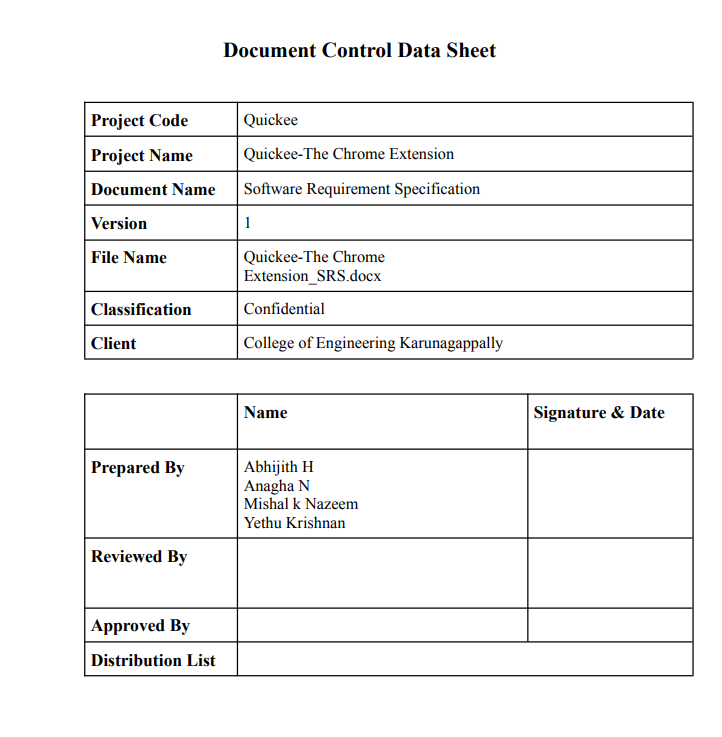
\includegraphics[scale=0.9]{figures/Screenshot (28).png}
\end{figure}

\begin{figure}[h!]
  \centering
  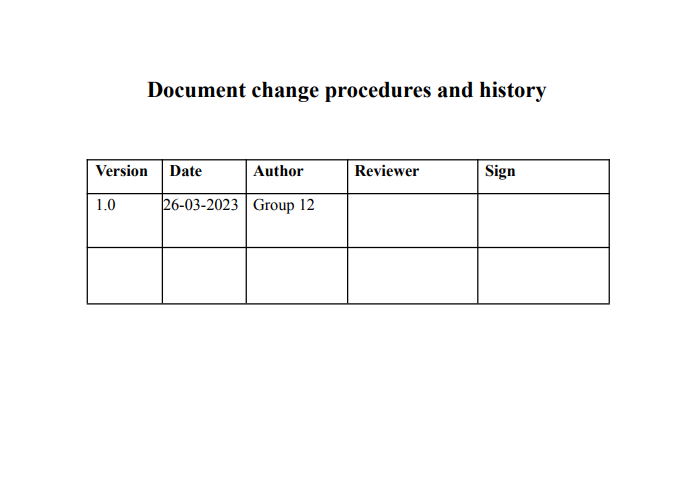
\includegraphics[scale=0.9]{figures/Screenshot (29).png}
\end{figure}
 %Unless essential Do not edit this tex file



%%********************Certificate*******************

% To print name of only the project coordinator 1 in the certificate page
\include{certificate1} 

% To print names of both the project coordinators in the certificate page
%%==================================certificate2.tex================================
% To print names of both the seminar coordinators in the certificate page
\newenvironment{certificate2}

\newpage
\begin{center}	
	%\vspace{1.5cm}
	
	\textbf{DEPT. OF ELECTRONICS \& COMMUNICATION ENGINEERING}	
	\textbf{COLLEGE OF ENGINEERING}	
	\textbf{KARUNAGAPPALLY}
	
	\textbf{\acadyear} 
\end{center}

\begin{center}
	\includegraphics[scale=0.5]{cet_logo}	
\end{center}
\begin{center}
	\textbf{CERTIFICATE}
\end{center}

This is to certify that the report entitled \textbf{\title} submitted by \textbf{\author} \hspace*{2pt}(\rollno), to the APJ Abdul Kalam Technological University in partial fulfillment of the B.Tech.\ degree in \branch \hspace*{2pt} is a bonafide record of the seminar work carried out by him under our guidance and supervision. This report in any form has not been submitted to any other University or Institute for any purpose.


\begin{singlespace}
	\vspace*{2cm}
	\begin{table}[h!]
		\centering
		\begin{tabular}{p{7cm} p{0.9cm} p{7cm}} 
			\textbf{\guide} && \textbf{\semcordinatorA} \\
			(Seminar Guide) &&  (Seminar Coordinator)\\
			\guidedes & & \semcordinatorAdes\\ 
			\deptabbr && \deptabbr\\ 
			\college & &\college\\
			\collegeplace && \collegeplace\\
		\end{tabular}
		
	\end{table}
	
	\vspace*{1.3cm}
	
	\begin{center}
		\begin{tabular}{p{7cm} p{0.9cm} p{7cm}} 
			%\hline
			\textbf{\semcordinatorB} && \textbf{\hod} \\
			\semcordinatorBdes & & \hoddes\\ 
			\deptabbr && \deptabbr\\ 
			\college & &\college\\
			\collegeplace && \collegeplace\\
		\end{tabular}
	\end{center}
\end{singlespace}

\thispagestyle{empty}



 %Please uncomment this and comment the previous line

%%***************************************************


\include{declaration} %Unless essential Do not edit this tex file

\pagenumbering{roman} 

%%********************************Abstract***********************
\include{abstract} % Please type in the abstract in this tex file abstract.tex

%%***************************************************
% Default Acknowledgement page
\include{acknowledgement}  %Unless essential Do not edit this tex file


%%***************************************************
%%**If you have only one seminar coordinator faculty member
% please comment the above line and uncomment this line

%\include{acknowledgement1}  %Unless essential Do not edit this tex file
%*******************************************************************

\thispagestyle{empty}
\newpage
    
%%**********************Table of Contents***********************
\tableofcontents

\include{symbol} %List of Symbols (Optional) comment if not required.
% symbold may be added in the file symbol.tex

%%********************Body of the report**********
% Arabic numbering is used in the body of the report

\cleardoublepage
\setcounter{page}{1}
\pagenumbering{arabic}
\begin{document}

\textbf{List of Tables}
\begin{align*}
    
\begin{flushleft}
    

 Table 1.1 Glossary 
\newline Table  3.1 User Login Information 
\newline Table 3.2 Personal Information 
\newline Table 4.1 Software Requirements 
 \newline Table 4.2 List of Actors 
\newline Table 4.3 Use Cases 
\newline Table 4.4 Functional Requirements To Use Cases Mapping 
\newline Table 4.5 UC1 
\newline Table 4.6 UC2 
\newline Table 4.7 UC3 
\newline Table 4.8 UC4 
\newline Table 4.9 UC5 
\newline Table 4.10 UC6 
\newline Table 4.11 UC7 
\newline Table 4.12 UC8 
\vspace{40}

\textbf{List of Figures}
\begin{align*}
    \begin{flushleft}
        
    
\newline Figure 2.1 QUICKEE System Environment 
\newline  Figure 4.1 QUICKEE Use Case 
 \newline Figure 6.1 Class Diagram


%%********************Chapter 1**********
\chapter{Introduction}
\begin{flushleft}
    

 \section{Purpose}

In today’s world, we are using online references for every doubt.There are
problems of distraction and time conception while doing traditional
referencing.This new system named ‘SenseAI’ adds a pinch of speed and
optimism to your online referencing. It provides environment to clear word wise
and topic wise immediate doubt clearances within the webpages by connecting the
user to ai.The intended audiences are vast.Mainly focuses on the people who
wants optimistic clearance of every topic being referenced and those who want
time management.These can be individuals,companies, even automated
programmes ,companies etc. The user can dictate a specific word or a paragraph
from the reference page to get explained by open ai . The purpose of this Software
Requirements Specification document is to figure out all the functions and
specifications of ‘SenseAI’.Besides it contains all the requirements specified . It
will explain the purpose and features of the system,what the system will do ,and
the constraints under which it must operate.This document is intended for both
consumers and the developers of the system.
\newpage
\section{ Intended Audience}


The intended Audience of the project is people who need productivity in
work and learning .
\section{ Scope of Project}

The existing system is a website . In the existing system , users
range from common people to scholars and researchers.When they need
the AI they need to go to the website and type in the prompt which causes
some time delay between fetching the required answer



  \underline{\textbf{Drawbacks}}

Time consuming
There is no website for accessing all the services at a single page
The techniques and UI can be confusing to common people
The proposed system is much more efficient than the existing
system. This is a Google Chrome extension which helps users to find the
answers to their queries much more easier ,timely and efficiently .The
extension acts as a one stop for all OpenAI products

\underline{\textbf{Advantages}}

Less time consuming
Easy, efficient and simple
Give quick and efficient service to users
High speed response to the users
Registration for every individual who are willing to donate

\section{Glossary}
 

\begin{table}[h] % Use the table environment to create a table
\caption{ Glossary} % Use \caption to specify the table name
\centering % Center the table
\begin{tabular}{|p{6.5cm}|p{7cm}|}
\hline
\textbf{Term} & 
\textbf{Definition} \\
\hline
SenseAI-An extension
to boost productivity &
SenseAI is a ChatExtension developed using API platform
and it aim to streamline communication and provide users
more functionalities\\
\hline
User &
A user of the SenseAI can be Consumer\\
\hline
Database &
Collection of all the information about the users and their
previous queries\\
\hline
Software Requirements
Specification &
A document that completely describes all of the functions of a
proposed system and the constraints under which it must
operate . For example,this document.\\
\hline
\end{tabular}
\end{table}\\
 \section{References}

 \section{Overview of Document}

The Overall Description section of this document gives an overview of the
functionality of the Chrome Extension. It describes the informal requirements and
is used to establish a context for the technical requirements specification in the
next chapter.
 \par The third chapter, Requirements Specification section, of this document is
written primarily for the developers and describes in technical terms the details of
the functionality of the Chrome Extension. Both sections of the document describe
the same software product in its entirety, but are intended for different audiences
and thus use different language

\end{flushleft}
 % Please comment this line and type in the introduction chapter


\chapter{Overall Description}
\begin{flushleft}
    

    
\section{System Environment}

The project Quickee involves a single user, the person who uses the
services offered by the extension .. In order to login, user has to first register by
providing the desired user-ID and password. Provided user-IDs and passwords by
the users are maintained in a database. NoSQL database is used to maintain a
database. Then the user logins in to the application by giving user-ID and
password provided during the registration process. IndexedDB is used to connect
the application with the database.


  \vspace{20pt}

\documentclass{}

\begin{document}



 
\setcounter{secnumdepth}{4}

User login sequence will be as follows:

\begin{itemize}
    \item The user registers by providing a user-ID and password (credentials). The user is prompted to enter user credentials.
    \item If the user enters correct credentials, then they get access to the application and can view their personal details and donation details. 
\end{itemize}

\vspace{20}
\newpage
\begin{figure}
    \centering
    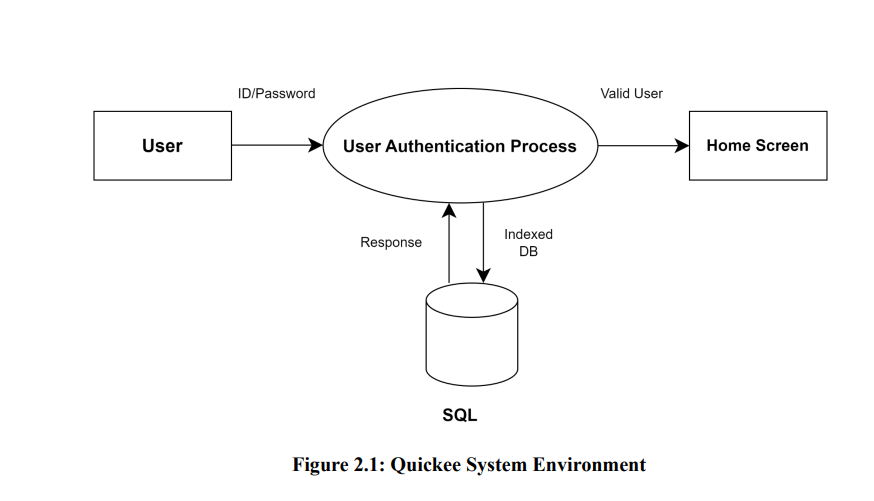
\includegraphics[scale = 0.8]{ figures/Screenshot (42).png}
    
    \label{fig:my_label}
\end{figure}
\section{product perspective}

\text{}{The project Quickee involves only one user and the user can access all the
services provided by the extension}


\section{product functions}
\text{}{The project Quickee involves only one user and the user can access all the
services provided by the extension}
\subsection{Login}
\textit{}The user logins in to the application by giving user-ID and password.
\subsection{User Management}
\textit{}To design front-end forms according to user specifications was like
adding new users. This module deals with user information details.
  \subsubsection{New User Acqusition}
  \textit{The proposed software allows the end user to add the new user with his personal
details}
\subsubsection{Signing out of user}
\textit{}The user can Sign Out of the Extension as he/she please.
\subsubsection{Deleting User Accouunt}
\textit{}User can delete their account on their discretion.All the user information
stored will be concurrently deleted
\subsubsection{Access Previous Queries}
\textit{}Users can access the history section to view their previous queries.
\subsection{Extension Services}
\textit{}This sub module is used to maintain the details of the blood bank. This
module also can update data of blood availability
\subsubsection{Image Generation}
\textit{}This sub module is used to generate comic style images for the sentences
selected in the web browser
\subsubsection{Summarization}
\textit{}This sub module is used to summarise the selected paragraph into a
smaller, much concise version of the original.
\subsubsection{Text Generation}
\textit{}This sub module is allowed to generate text based on the sentence selected
by the user (Generated text can be answers to questions,can be letters etc).

\subsubsection{Code Generation}
\textit{}This sub module is allowed to generate code for the problem which is
selected by user . The language is preselect but can be changed by user.
\section{User Characteristics}
\textit{}There is only a single user for the system
\subsection{Users}
\textit{}Only after the login process, the rest of the application is made available
to the user. In order to login, user has to first register by providing desired user-ID
and password. Consumers can update personal information , access the services.
\section{Development Environment}
\textit{}Development environment is as follows. Final decision on the
development environment shall be taken during the design phase.

\vspace{20pt}

\textit{}React.js.

\vspace{20pt}

\textit{}Database: NoSQL.
\section{Constraints}
\begin{enumerate}[a)]
    \item \bold{} Regulatory Policies:NA
    \item  Hardware Limitations: NA
    \item Interfaces to other application: API calls to openAI
    \item Parallel operations: NA
    \item  Audit Functions: NA
    \item Control Functions: NA
    \item Safety and Security Considerations: The password and a valid username are the
security issues. The backup process at the server side shall satisfy data protection.
    \item Reliability Requirements:Total number of bugs in the system shall not exceed
1  percentage of the total line number of code,except connection reliability,which is out of
    \item  Criticality of the Application: The server applications shall be available 365
days.

\end{enumerate}

\section{ Assumptions and Dependencies}
\textit{}Since the SENSEAI is only accessible through the Internet it is assumed that
the end user has a connection to the Internet. It is also assumed that the user has a
web browser able to display/installing the SENSEAI Extension.




\chapter{Requirements Specification}
\usepackage{}
\section{External Interface Requirements}
\subsection{User interfaces}
\textit{}The system will allow access using web browsers . Most common
browsers with JavaScript enabled will be supported.The system can be installed
on to consumers web browser from the web store.

\vspace{20pt}

At first users has to register for an account , then user can login to their
account to access their services and previous query history.
\subsection{Hardware Interfaces}
\textit{}There are no external hardware interface requirements for SENSEAI.
\subsection{Software interfaces}
\textit{}There are no external software interface requirements for SENSEAI.
\subsection{Communication Interfaces}
\textit{}There are no external communications interface requirements for SENSEAI.
\section{Functional Requirements}
\subsection{Login Management}
\subsubsection{Login Information}
\textit{}The system shall maintain at a minimum the information in Table 3.1.
\vspace{20pt}
\begin{table}
    \centering
    \caption{User Login Information}
    \begin{tabular}{|c|c|c|}
        \hline
        Property & Mandatory & Explanation \\
        \hline
          Email & Yes & Email for the login process \\
        \hline
        Password & Yes & Password for the login process
 \\
        \hline

    \end{tabular}
\end{table}
\subsubsection{ User login Operation}
\textit{}By giving the user name and password the user can login into the
SENSEAI and can access the services and access their history.

\subsection{User Management}
\subsubsection{Personal Information of donors}
\textit{}The system shall maintain at a minimum the information in Table 3.2
\begin{table}
    \centering
    \caption{Personal Information}
    \begin{tabular}{|c|c|c|}
        \hline
        Property & Mandatory & Explanation \\
        \hline
          Email & Yes & Name of the user \\
        \hline
        Password & Yes & Email of the user
 \\
        \hline


    \end{tabular}
\end{table}

\subsubsection{ New Consumer Acquisition Operation}
\textit{}Here new user can register into the SENSEAI with his personal details
and by providing a email and password.
\subsection{Access Services}
\subsubsection{Preset prompts}
Here the user can access the services based on the preset default prompts.
\subsubsection{Custom prompts}
\textit{}Here the user can set their own custom prompt which can be used to access
the services.

\chapter{System Features}
\textit{}This section gives the details of system features and functions identified as
different use cases relevant for various users (or actors) of the system. The
following sections group and specify the use cases.
\section{Table 4.1: Software Requirements}
\begin{table}[h]
    

    \hspace*{-3cm}
    \begin{tabular}{|c|c|c|c|}
        \hline
 R.No & Requirements & Requirement Type & Priority \\
        \hline
 R1 & The system must allow the user to generate images based on text selection & STRQ1 & High \\
        \hline
 R2 & The system must allow the user to generate text based on text selection & STRQ2 & High \\
        \hline
R3 & The system must allow the user to generate code based on text selection & STRQ3 & High \\
        \hline
R4 & The system must allow the user to summarise text selection & STRQ4 & High \\
        \hline
 R5 & The system must allow the user to set custom prompts & STRQ5 & High \\
        \hline
 R6 & The user can view their previous queries & STRQ6 & High \\
        \hline
R7 & System shall provide authentication to avoid unauthorised access & STRQ7 & High \\
        \hline
        
R8 & System has to be web browser extension & FEAT1 & High \\
        \hline
R9 & System should be developed as Javascript as front end and NoSQL as backend & FEAT2 & High \\
        \hline 
R10 & Use CAPTCHA to reduce automated logins & FEAT3 & Low \\
        \hline
    \end{tabular}
\end{table}

\section{List of Actors}
\documentclass{}

\begin{document}

\begin{tabular}{|c|c|c|}
  \hline
  Actor No. & Actor  & Description \\
  \hline
  AIU & User & User can access all the services provided by the
Extension \\
  \hline
\end{tabular}


 \section{List of Use Cases}

\begin{figure}[]
  \centering
  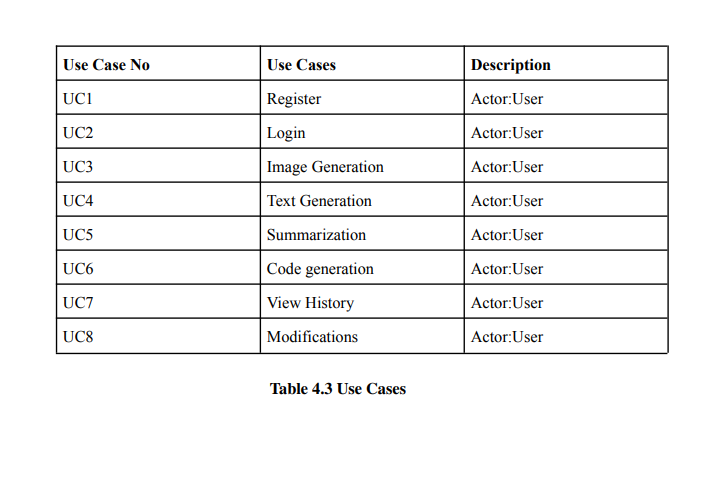
\includegraphics[scale=0.9]{figures/Screenshot (30).png}
\end{figure}

\newpage
\section{Mapping Functional Requirements to Use Cases}
\begin{figure}[h]
  \centering
  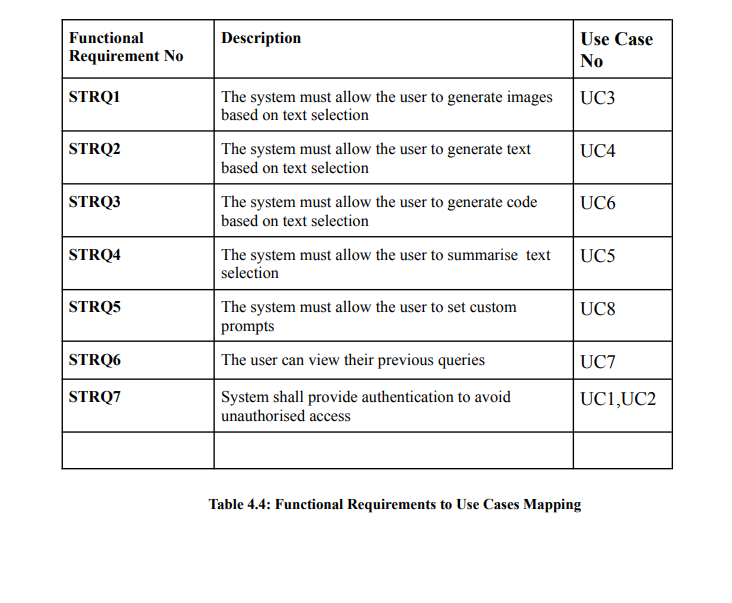
\includegraphics[scale=0.9]{figures/Screenshot (31).png}
\end{figure}
\newpage
\section{Use Case Diagram}


\begin{figure}[h]
  \centering
  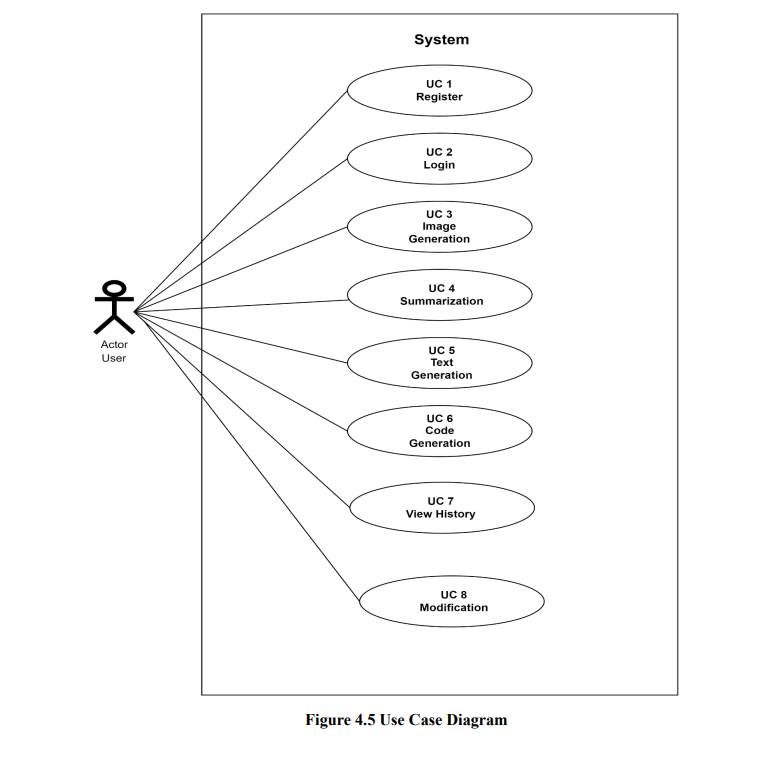
\includegraphics[scale=0.9]{figures/Screenshot (32).png}
  
\end{figure}
\subsection{Use Case-1 :Register}
  \begin{figure}[h]
        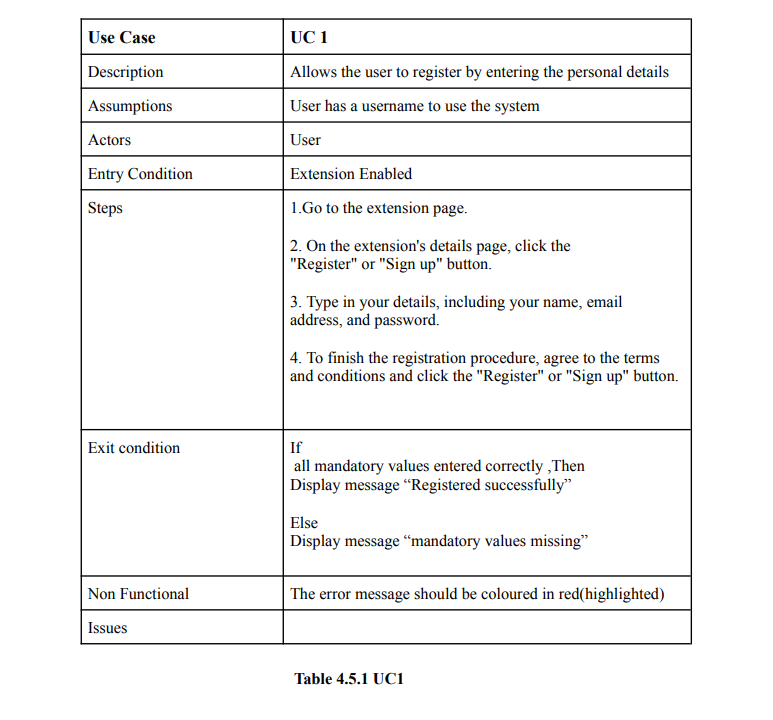
\includegraphics[scale=0.9]{figures/Screenshot (33).png}

   \end{figure}
   \subsection{Use Case-2:Login}

    \begin{figure}[h]
        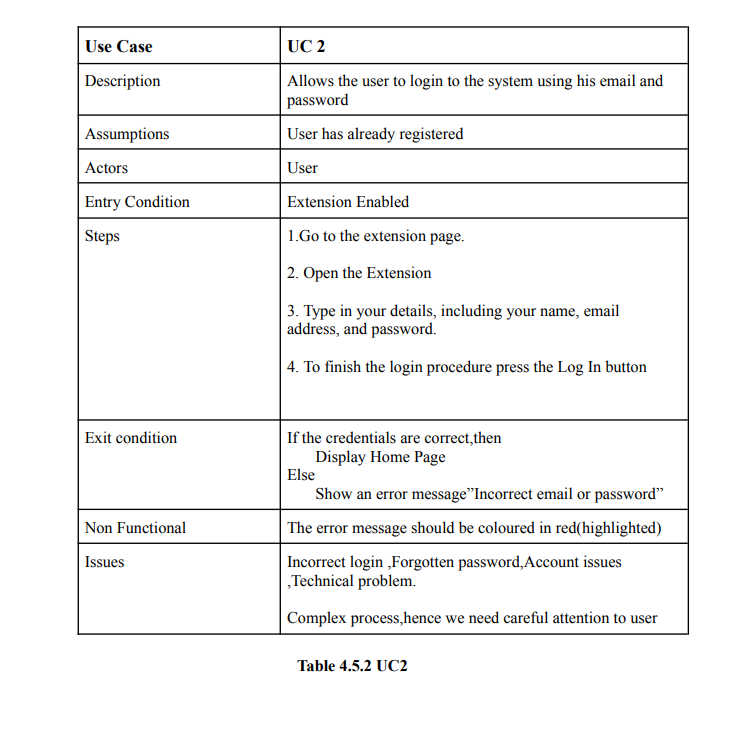
\includegraphics[scale=0.9]{figures/Screenshot (34).png}

   \end{figure}
   \subsection{ Use Case-3: Image Generation}
 \begin{figure}[h]
        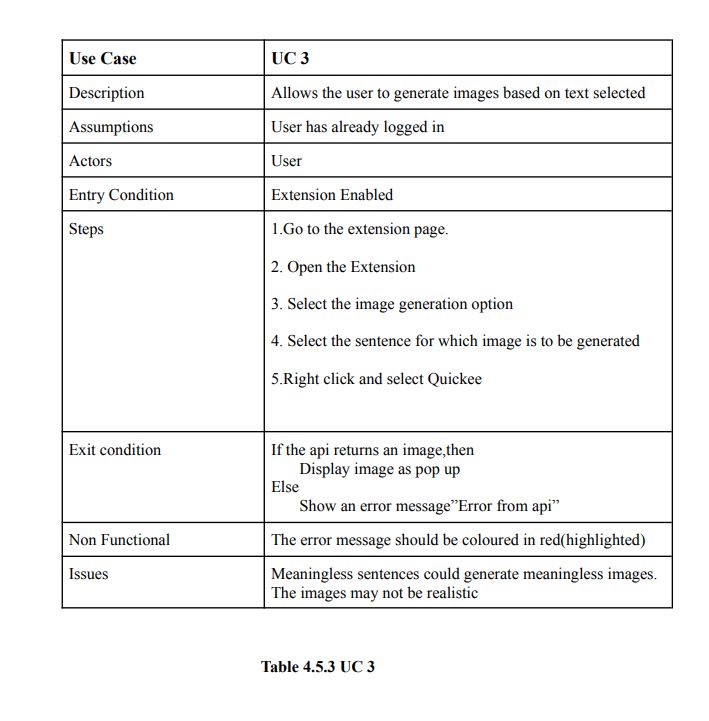
\includegraphics[scale=0.9]{figures/Screenshot (35).png}

   \end{figure}
    \subsection{ Use Case-4: Text Generation}
 \begin{figure}[h]
        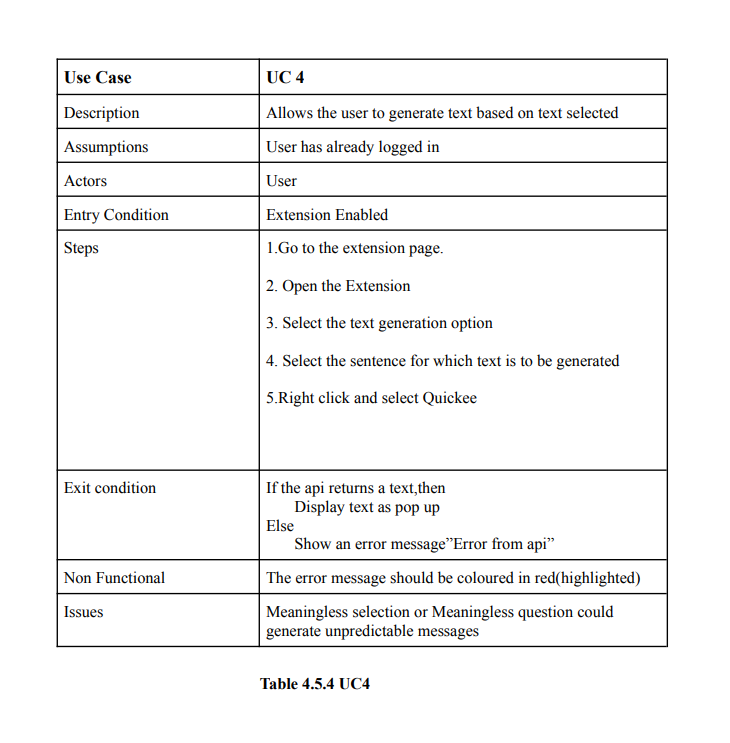
\includegraphics[scale=0.9]{figures/Screenshot (40).png}

   \end{figure}
    \subsection{Use Case-5: Summarization }
 \begin{figure}[h]
        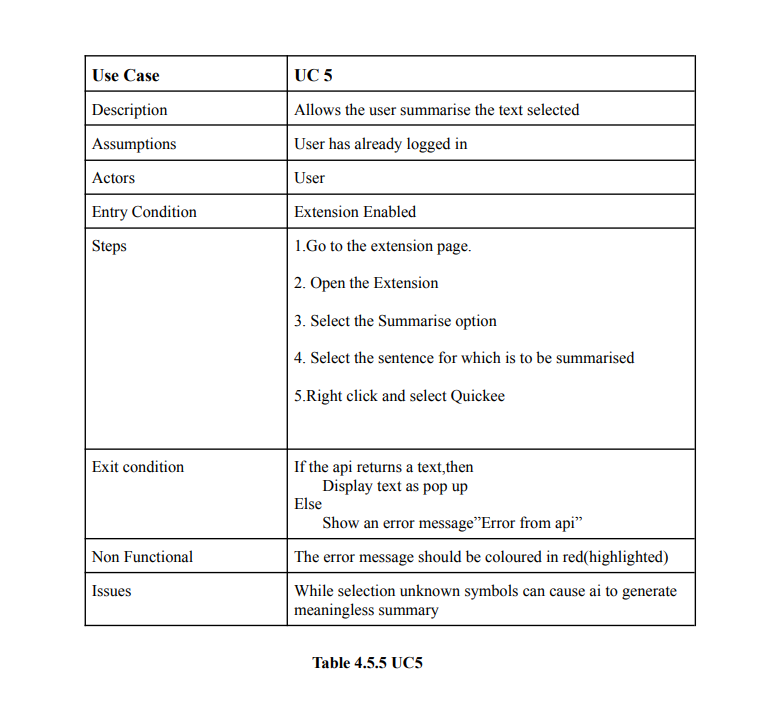
\includegraphics[scale=0.9]{figures/Screenshot (39).png}

   \end{figure}
     \subsection{ Use Case-6: Code Generation}
 \begin{figure}[h]
        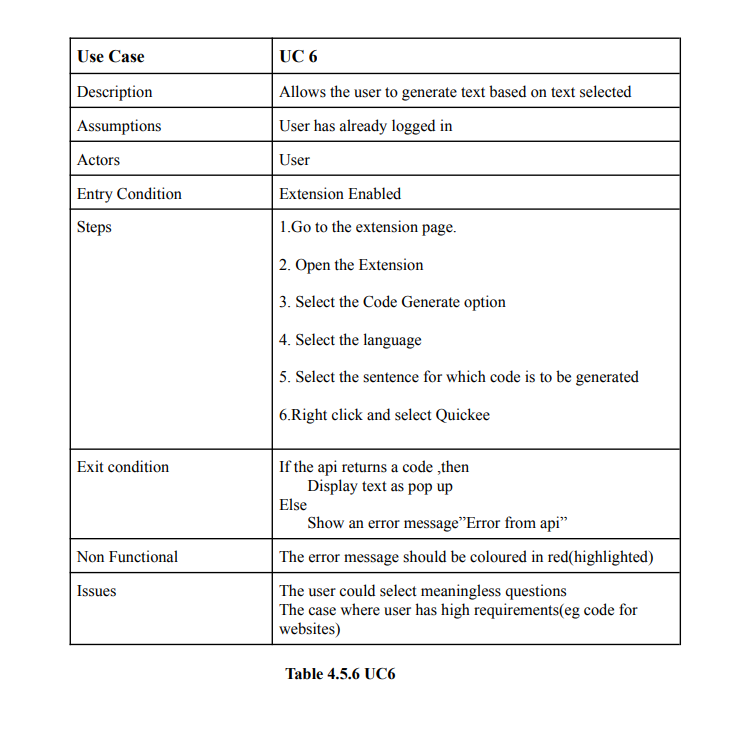
\includegraphics[scale=0.9]{figures/Screenshot (36).png}

   \end{figure}
   \subsection{ Use Case-7: View History}
    \begin{figure}[h]
       
 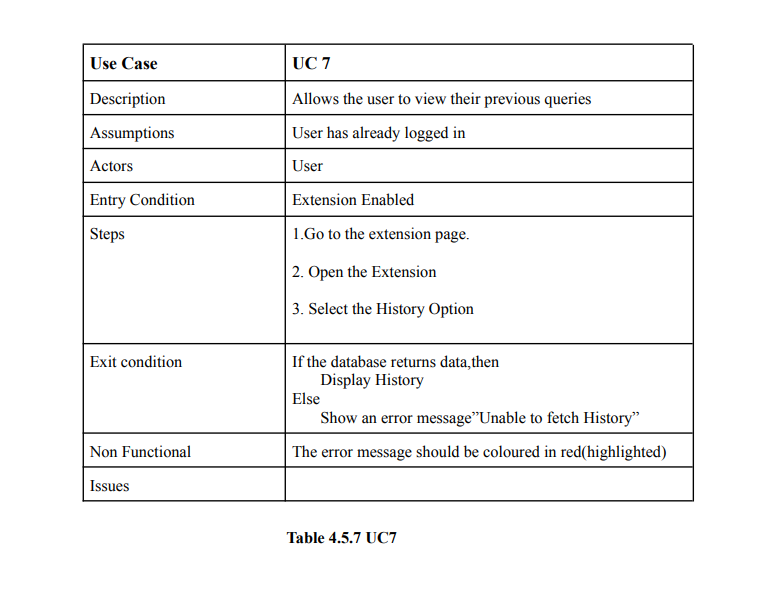
\includegraphics[scale=0.9]{figures/Screenshot (37).png}

   \end{figure}
   \subsection{ Use Case-8:  Modification}
           \begin{figure}[h]
        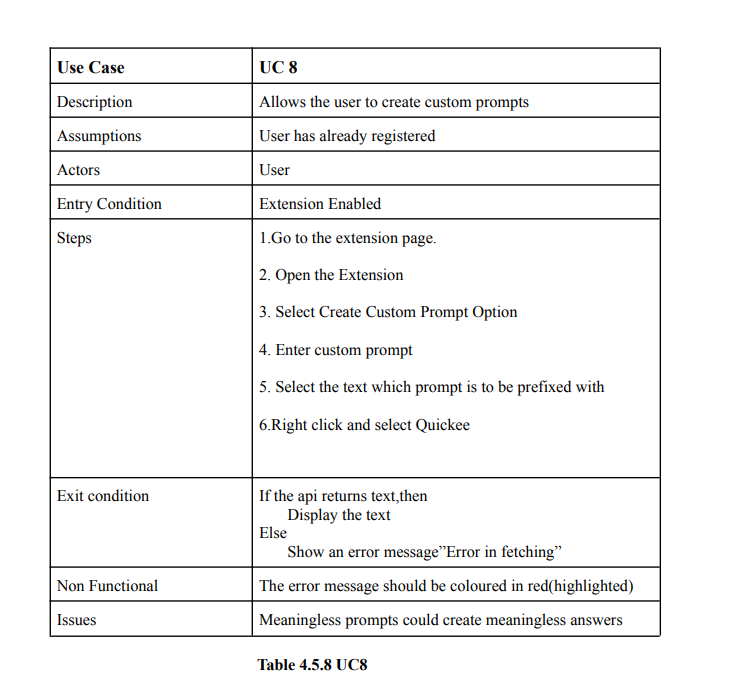
\includegraphics[scale=0.9]{figures/Screenshot (38).png}
   \end{figure}

\chapter{Other Non functional Requirements}
\textit{}In software engineering non-functional requirements are requirements
which specify criteria that can be used to judge the operation of a system, rather
than specific behaviours. This should be contrasted with functional requirements
that specify specific behaviour or functions. Non-functional requirements are
often called qualities of a system. Other terms for non-functional requirements are
"constraints", "quality attributes", "quality goals" and "quality of service
requirements". Qualities, of Non-functional requirements can be divided into two
main categories. Execution qualities, such as security and usability, are observable
at run time. Evolution qualities, such as extensibility and scalability, embody in
the static structure of the software system.




\section{Performance Requirements}
\lipsum[The server on which this system will be running is expected to be available
at all hours of the day to provide full time accessibility. The system is developed
based on the client server architecture, a request-response paradigm and is
implemented with the help of a Javascript and it uses NoSQL server as back end.
Major performance requirements are:
All prompts should be loaded within 60 seconds.
The system should provide proper authentication.] % Please comment this line and type in the content


\section{Security Requirements}
\lipsum[The access to the software application will be restricted to the authorised
users identified by a valid email and password. New users can register or sign up
to the system with personal details. CAPTCHA will be included to reduce automated
login. Error messages will be displayed in the case of errors during the system access.] % Please comment this line and type in the content

\chapter{ Uml Diagrams}
\section{ Class diagram}
\textit{}Class diagrams are used to describe the structure of a system. Class
diagrams describe the system in terms of objects, classes, attributes, operations
and their associations. Objects are instances of the classes. In UML classes are
depicted by boxes composed of three compartments. The top compartment
displays the name of the class. The centre compartment displays its attributes,
and the bottom compartment displays operations. A link represents the
connection between the classes.
  \begin{figure}[h]
        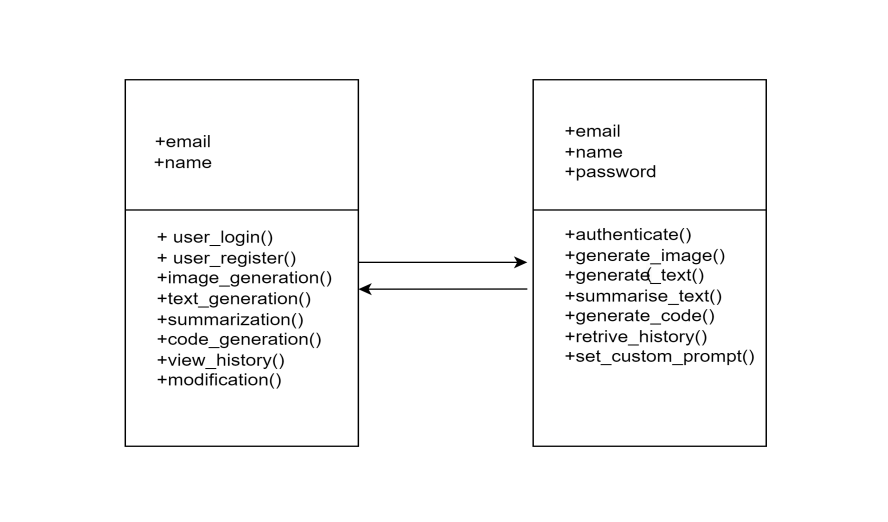
\includegraphics[scale=0.8]{figures/Screenshot (41).png}
   \end{figure}
   \section{ Sequence Diagram}
\textit{}Sequence diagram is an Interaction Diagram that describes the
patterns of communication among a set of interacting objects. An
object interacts with another object by sending messages. The
reception of message by an object triggers the execution of a
method, which in turn may send messages to other objects.
Arguments may be passed along with a message and are bound to
parameters of the executing method in the receiving object
.Sequence Diagrams represent the objects participating in the
interaction horizontally and time vertically.   
 \section{ State Chart Diagrams}
 \textit{ }State chart diagrams describe the dynamic behaviour of an
individual object as a number of states and transition between these
states. A state represents particular set of values for an object.
Given a state, a transition represents a future state the object can
move to and the conditions associated with the change of state. A
state is represented by a rounded rectangle. A transition is depicted
by open arrows connecting two states. States are labelled with their
name. A small solid black circle indicates the initial state. A circle
surrounding a small solid black circle indicates a final.
\end{document}

